\chapter{Исследовательская часть}

\section{Технические характеристики}
Замеры проводились на микроконтроллере STM32F767 Nucleo-144 с установленным  micropython.

Микроконтроллер имеет процессор Arm Cortex-M7 216 МГц и 512 КБ оперативной памяти.

\section{Временные характеристики}
Временные характеристики алгоритмов замерялись при вариативном линейном размере квадратных матриц, при этом каждый размер матрицы считался количество раз, которое позволяла память платы. Количество измерений для каждого размера указано в последнем столбце таблицы. На каждое измерение генерировались две случайные матрицы заданного размера и подавались на вход всем 3-м функциям. Результаты замеров представлены в таблице \ref{tbl:time_algo}



\begin{table}[ht]
	\small
	\begin{center}
		\begin{threeparttable}
			
			\caption{Временные характеристики}
			\label{tbl:time_algo}
			\begin{tabular}{|p{0.10\textwidth}|p{0.15\textwidth}|p{0.15\textwidth}|p{0.20\textwidth}|p{0.15\textwidth}| }
				\hline
				\centering{Размер, элементы} & \centering{Стандартный алгоритм, мс} & \centering{Алгоритм Винограда, мс} & \centering{Оптимизированный алгоритм Винограда, мс} & \centering{Количество замеров} \\
				\cr
				\hline
				\multicolumn{1}{|r|}{5}& \multicolumn{1}{|r|}{1} & \multicolumn{1}{|r|}{1} & \multicolumn{1}{|r|}{1} & \multicolumn{1}{|r|}{20} \\
				\hline
				\multicolumn{1}{|r|}{10} & \multicolumn{1}{|r|}{8} & \multicolumn{1}{|r|}{8} & \multicolumn{1}{|r|}{6} & \multicolumn{1}{|r|}{20} \\
				\hline
				\multicolumn{1}{|r|}{15} & \multicolumn{1}{|r|}{26} & \multicolumn{1}{|r|}{26} & \multicolumn{1}{|r|}{21} & \multicolumn{1}{|r|}{20} \\
				\hline
				\multicolumn{1}{|r|}{20} & \multicolumn{1}{|r|}{61} & \multicolumn{1}{|r|}{61} & \multicolumn{1}{|r|}{48} & \multicolumn{1}{|r|}{20} \\
				\hline
				\multicolumn{1}{|r|}{25} & \multicolumn{1}{|r|}{117} & \multicolumn{1}{|r|}{120} & \multicolumn{1}{|r|}{96} & \multicolumn{1}{|r|}{20} \\
				\hline
				\multicolumn{1}{|r|}{30} & \multicolumn{1}{|r|}{201} & \multicolumn{1}{|r|}{212} & \multicolumn{1}{|r|}{170} & \multicolumn{1}{|r|}{10} \\
				\hline
				\multicolumn{1}{|r|}{35} & \multicolumn{1}{|r|}{318} & \multicolumn{1}{|r|}{338} & \multicolumn{1}{|r|}{274} & \multicolumn{1}{|r|}{10} \\
				\hline
				\multicolumn{1}{|r|}{40} & \multicolumn{1}{|r|}{474} & \multicolumn{1}{|r|}{514} & \multicolumn{1}{|r|}{421} & \multicolumn{1}{|r|}{5} \\
				\hline
				\multicolumn{1}{|r|}{45} & \multicolumn{1}{|r|}{671} & \multicolumn{1}{|r|}{752} & \multicolumn{1}{|r|}{619} & \multicolumn{1}{|r|}{5} \\
				\hline
				\multicolumn{1}{|r|}{50} & \multicolumn{1}{|r|}{919} & \multicolumn{1}{|r|}{1010} & \multicolumn{1}{|r|}{828} & \multicolumn{1}{|r|}{3} \\
				\hline
			\end{tabular}	
		\end{threeparttable}
	\end{center}
\end{table}

Полученные замеры также можно увидеть на графике (\ref{fig:time_graph}):

\begin{figure}
	\centering
	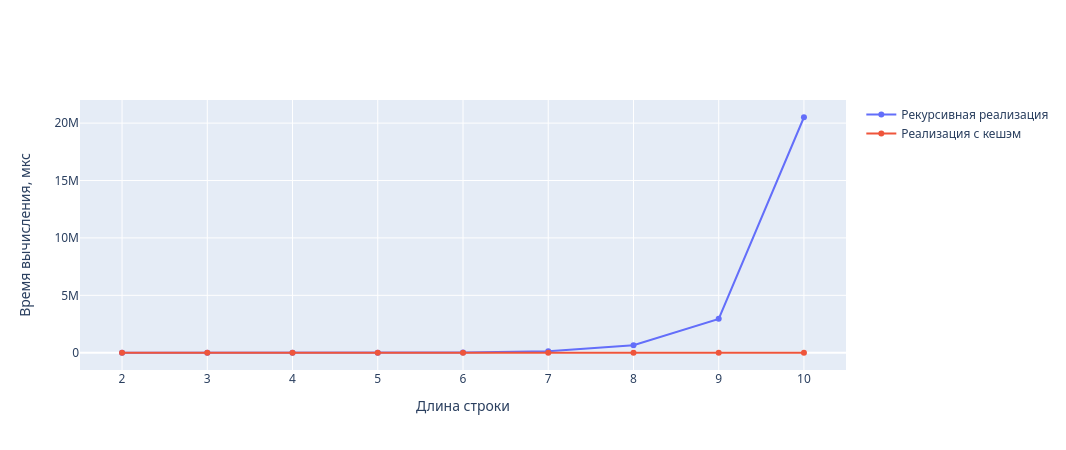
\includegraphics[width=0.9\textwidth]{time}
	\caption{График зависимости времени работы алгоритмов от линейного размер квадратной матрицы}
	\label{fig:time_graph}
\end{figure}

Как видно из таблицы (\ref{tbl:time_algo}) и графика (\ref{fig:time_graph}), оптимизированный алгоритм эффективнее двух других.

\pagebreak

\section{Вывод}

В данном разделе было проведено исследование временных и алгоритмов умножения матриц.

В результате исследования было выявлено, что самым эффективным оказался алгоритм Винограда с оптимизацией, при этом алгоритм Винограда без оптимизации оказался самым медленным. Результаты исследования соотносятся с трудоёмкостями алгоритмов, рассчитанным в формулах \ref{eq:f-std}–\ref{eq:ovin}.

\clearpage
